\graphicspath{{modelling/fig/}}
{
\tikzset{external/figure name/.add={modelling/}{}}

\chapter{Modelling}
\label{chap:modelling}

\paragraph
In this chapter, a non-linear mathematical model of a multirotor with a suspended payload will be derived.
The model will be based on the multirotor named \emph{Honeybee}, which was built by \citet{Grobler2020}.
% A simulation environnement based on this model will be used to simulate the multirotor-payload system in subsequent chapters.

\paragraph
The chapter starts by defining the coordinate frames and types of rotations used in this work.
After a discussion of the different forces and moments acting on this vehicle, 
a \gls{6DOF} model of the multirotor vehicle will be derived.
The derivation of the suspended payload model will also be shown.
Finally, practical flight data will be used to verify the simulated mathematical model.

\FloatBarrier\section{Coordinate frames}

    \paragraph
    Honeybee is quadrotor vehicle, which is a type of multirotor with four propellers.
    The quadrotor X-configuration is considered in this work.
    Figure~\ref{fig:coord_frames} shows the quadrotor schematic and the two coordinate frames used to describe this system.
    
    \begin{figure}[htb]
        \centering
        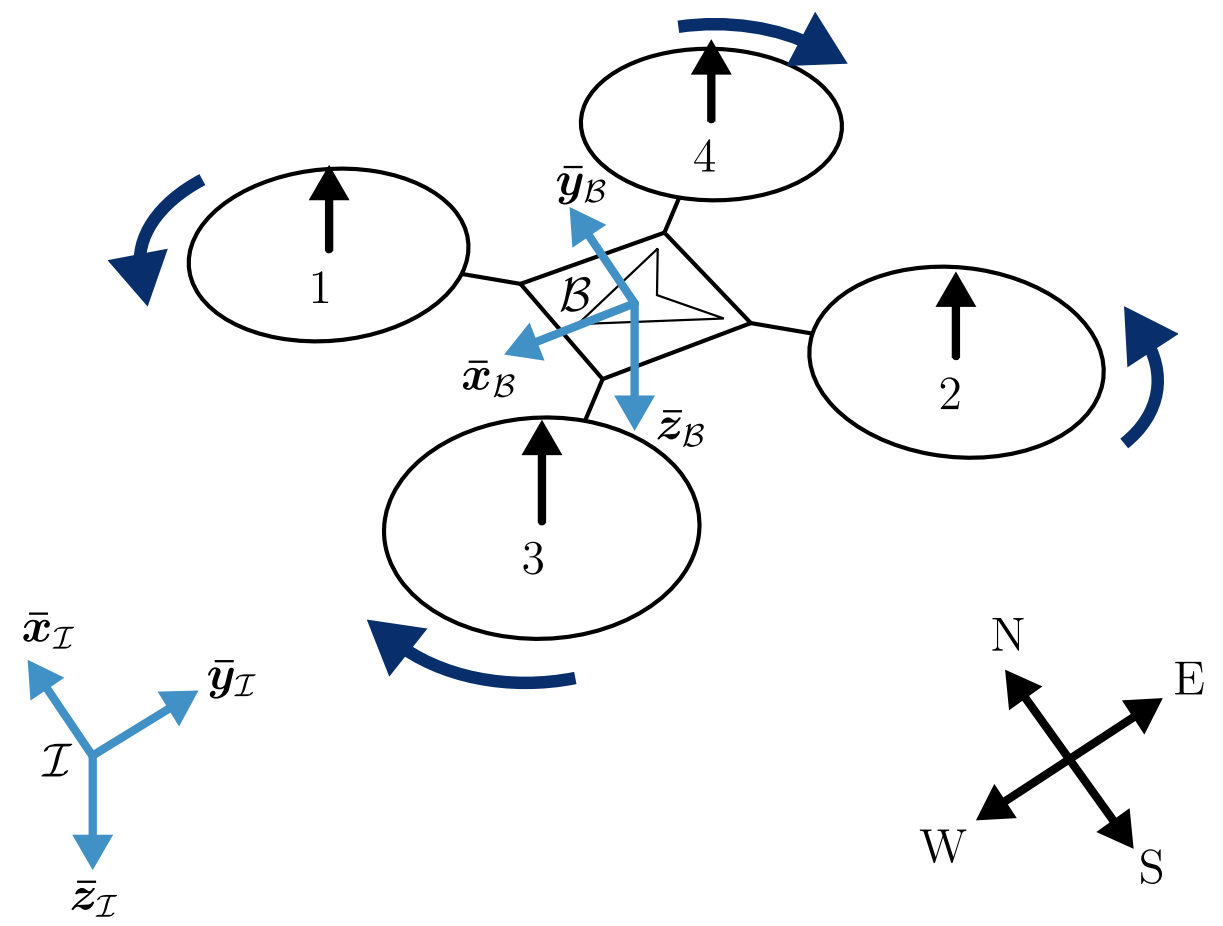
\includegraphics[width=0.6\linewidth]{modelling/fig/coord_frames}
        \caption{Inertial and body coordinate frames of a quadrotor \cite{Erasmus2020}}
        \label{fig:coord_frames}
    \end{figure}

    \paragraph
    The inertial frame is denoted by $ \mathcal{I} = \{ \bm{\bar{x}}_\mathcal{I}, \bm{\bar{y}}_\mathcal{I}, \bm{\bar{z}}_\mathcal{I} \} $ and describes a \gls{NED} axis system.
    The $x$, $y$, and $z$ axis, align with the North, East, and Down inertial directions respectively.
    The inertial frame assumes a flat, non-rotating earth since the multirotor travels small distances in comparison to the curvature of the earth.
    The origin of this frame is fixed at the takeoff location of the multirotor.

    \paragraph
    The body frame is denote by $ \mathcal{B} = \{ \bm{\bar{x}}_\mathcal{B}, \bm{\bar{y}}_\mathcal{B}, \bm{\bar{z}}_\mathcal{B} \} $ and is fixed to the multirotor body.
    The origin of this frame is at the \gls{CoM} of the vehicle and the $x$, $y$, and $z$ axes, align with the forwards, rightwards, and downwards directions of the multirotor body respectively.
    The body frame is defined by a translation and rotation relative to the inertial frame.
    % The position of the multirotor \gls{CoM} in the inertial frame is denoted as $P = [P_N~~P_E~~P_D]^T$. 
    % This represents the translation of the body frame relative to the inertial frame.
    The mathematical representation of rotations is be discussed in the section below.

\FloatBarrier\section{Rotations}
    
    \paragraph
    The rotation of the body frame relative to the inertial frame is referred to as the attitude of the multirotor.
    In this work, the attitude is defined in terms of Euler angles or quaternions.

    \FloatBarrier\subsection{Euler angles}

        \paragraph
        Euler angles describe a \gls{3D} rotation as a sequence of three consecutive elementary rotations \cite{Brescianini2013}.
        The ZYX-sequence is commonly used for aircraft applications \cite{Brescianini2013} and is also used in this work.
        The order of rotations are:
        \begin{enumerate}
            \item Rotate the body frame about the $z$-axis by the yaw angle, $\Psi$.
            \item Rotate the resulting frame about the new $y$-axis by the pitch angle, $\Theta$.
            \item Rotate the resulting frame about the new $x$-axis by the roll angle, $\Phi$.
        \end{enumerate}

        \begin{figure}[!htbp]
            \centering
            \vspace{0.5cm}
            \def\svgwidth{\columnwidth}
            \scalebox{0.85}{\input{modelling/fig/Euler_rotations.pdf_tex}}
            \vspace{0.5cm}
            \caption{Illustration of Euler angles \cite{Slabber2020}}
            \label{fig:Euler_rotations}
        \end{figure}

        \paragraph
        Figure~\ref{fig:Euler_rotations} gives a simple illustration of the Euler-ZYX angles.
        For simplicity in the illustration, $\Theta$ and $\Phi$ are each shown as a pure pitch and roll angle, without a prior Euler rotation.

    \FloatBarrier\subsection{Quaternions}

        \paragraph
        Quaternions provide a way of representing a rotation with four parameters.
        An advantage of quaternions is that it does not have mathematical singularities like Euler angles do \cite{Brescianini2013}.
        A quaternion defines a \gls{3D} rotation as a single rotation about a fixed axis.
        This is parametrized by a rotation angle, $\alpha$, and a unit vector, $\vec{r}$.
        
        \paragraph
        A unit quaternion is defined as,
        \begin{equation}
            \bm{q} = [q_0~~q_1~~q_2~~q_3]^T = 
            \begin{bmatrix}
                q_0 \\ 
                \bm{q}_v
            \end{bmatrix}
            =
            \begin{bmatrix}
                \cos(\frac{\alpha}{2}) \\ 
                \vec{r} \sin(\frac{\alpha}{2} )
            \end{bmatrix} ,
        \end{equation}
        where $q_0$ is the magnitude component and $\bm{q}_v$ is the vector component of the quaternion.

        \paragraph
        A Euler-ZYX angle representation, $[\Theta~~\Phi~~\Psi]$, can be converted to a quaternion using \cite{Brescianini2013},
        \begin{equation}
            \bm{q}(\Theta, \Phi, \Psi) = 
            \left[\begin{array}{c}
                \begin{aligned}%[t]
                     \cos{\tfrac{\Phi}{2}} \cos{\tfrac{\Theta}{2}}  \cos{\tfrac{\Psi}{2}}    ~~ &+ ~~ \sin{\tfrac{\Phi}{2}}   \sin{\tfrac{\Theta}{2}}  \sin{\tfrac{\Psi}{2}} \\
                    -\cos{\tfrac{\Phi}{2}} \sin{\tfrac{\Theta}{2}}  \sin{\tfrac{\Psi}{2}}    ~~ &+ ~~ \cos{\tfrac{\Theta}{2}} \cos{\tfrac{\Psi}{2}}    \sin{\tfrac{\Phi}{2}} \\
                     \cos{\tfrac{\Phi}{2}} \cos{\tfrac{\Psi}{2}}    \sin{\tfrac{\Theta}{2}}  ~~ &+ ~~ \sin{\tfrac{\Phi}{2}}   \cos{\tfrac{\Psi}{2}}    \sin{\tfrac{\Psi}{2}} \\
                     \cos{\tfrac{\Phi}{2}} \cos{\tfrac{\Theta}{2}}  \sin{\tfrac{\Psi}{2}}    ~~ &- ~~ \sin{\tfrac{\Phi}{2}}   \cos{\tfrac{\Psi}{2}}    \sin{\tfrac{\Theta}{2}} \\
                \end{aligned}
            \end{array}\right] .
        \end{equation}

        \paragraph
        The inverse of a quaternion is defined as,
        \begin{equation}
            \bm{q}^{-1} = 
            \frac{ \begin{bmatrix} q_0 \\ -\bm{q}_v \end{bmatrix} }{ \sqrt{ {q_{0}}^{2} + {q_{1}}^{2} + {q_{2}}^{2} + {q_{3}}^{2} } } .
        \end{equation}

        \paragraph
        Furthermore, the multiplication of two quaternions, $\bm{q}$ and $\bm{q}^\prime$, is given by \cite{Brescianini2013}:
        \begin{equation}
            \bm{q} \cdot \bm{q}^\prime
            =
            Q( \bm{q} ) \bm{q}^\prime,
        \end{equation}
        where
        \begin{equation}
            Q( \bm{q} ) = 
            \left[\begin{array}{cccc}
                q_{0} &           - q_{1} &           - q_{2} &           - q_{3} \\
                q_{1} & \phantom{-} q_{0} &           - q_{3} & \phantom{-} q_{2} \\
                q_{2} & \phantom{-} q_{3} & \phantom{-} q_{0} &           - q_{1} \\
                q_{3} &           - q_{2} & \phantom{-} q_{1} & \phantom{-} q_{0}
            \end{array}\right] .
        \end{equation}

        \paragraph
        Successive rotations can therefore be represented mathematically by quaternion multiplication.
        These equations will be referred to and used in subsequent chapters.

\FloatBarrier\section{Multirotor model}

    \paragraph
    The multirotor is modelled as a \gls{6DOF} rigid body.
    This includes three translational and three rotational degrees of freedom.
    This modelling process is well described by \cite{Erasmus2020} and \cite{Slabber2020}, and the same general procedure is used here. 
    
    \paragraph
    The system parameters describing the physical properties of the multirotor is listed in Table~\ref{tbl:multirotor_params}.
    % These parameters are used in subsequent sections to derive a model of the multirotor.

    \begin{table}[!htbp]
        \renewcommand{\arraystretch}{1.1}
        \centering
        \caption{System parameters of the multirotor model.}
        \begin{tabularx}{0.66\linewidth}{@{}ll@{}}
            \toprule
            \textbf{Symbol}   & \textbf{Description} \\
            \midrule
                $m_Q$       & Mass of multirotor \\
                $d$         & Distance from \gls{CoM} to each motor\\
                $R_N$       & Virtual yaw moment arm \\
                $\tau$      & Motor-propeller pair time constant \\ 
                $I_{xx}$    & Mass moment of inertia about $\bm{\bar{x}}_\mathcal{B}$ \\ 
                $I_{yy}$    & Mass moment of inertia about $\bm{\bar{y}}_\mathcal{B}$ \\ 
                $I_{zz}$    & Mass moment of inertia about $\bm{\bar{z}}_\mathcal{B}$ \\ 
                $C_{Q_X}$   & Aerodynamic drag coefficient in $\bm{\bar{x}}_\mathcal{B}$ direction \\
                $C_{Q_Y}$   & Aerodynamic drag coefficient in $\bm{\bar{x}}_\mathcal{B}$ direction \\
                $C_{Q_Z}$   & Aerodynamic drag coefficient in $\bm{\bar{x}}_\mathcal{B}$ direction \\
            \bottomrule
        \end{tabularx}
        \label{tbl:multirotor_params}
    \end{table}

    % ?? Insert light rule under headings

    \paragraph
    The inertia tensor of the multirotor is defined as,
    \begin{equation} \label{eq:inertia}
        \bm{I_Q} = 
        \begin{bmatrix}
            I_{xx} & I_{xy} & I_{xz}\\
            I_{yx} & I_{yy} & I_{yz}\\
            I_{zx} & I_{zy} & I_{zz}
        \end{bmatrix}
        \approx
        \begin{bmatrix}
            I_{xx} & 0 & 0\\
            0 & I_{yy} & 0\\
            0 & 0 & I_{zz}
        \end{bmatrix}.
    \end{equation}
    The multirotor is assumed to be symmetrical about the $XZ$- and $YZ$-plane, therefore the inertia tensor can be approximated as a diagonal matrix as shown in Equation~\ref{eq:inertia}. 


    \paragraph
    The linear velocity and angular velocity of the multirotor within the body frame is denoted by,
    \begin{align}
        \bm{V_\mathcal{B}}          &= 
        \begin{bmatrix}
            V_{\mathcal{B}_X} & V_{\mathcal{B}_Y} & V_{\mathcal{B}_Z}\\
        \end{bmatrix}^T , \mbox{ and} \\
        \bm{\varOmega_\mathcal{B}}  &= 
        \begin{bmatrix}
            \varOmega_{\mathcal{B}_X} & \varOmega_{\mathcal{B}_Y} & \varOmega_{\mathcal{B}_Z}\\
        \end{bmatrix}^T.
    \end{align}
    Furthermore, the sum of forces and sum of moments acting on the multirotor in the body frame are denotes by,
    \begin{align}
        \bm{F_\mathcal{B}} = &
        \begin{bmatrix}
            F_{\mathcal{B}_X} & F_{\mathcal{B}_Y} & F_{\mathcal{B}_Z} \\
        \end{bmatrix}^T , \mbox{ and}\\
            \bm{M_\mathcal{B}} = &
        \begin{bmatrix}
            M_{\mathcal{B}_X} & M_{\mathcal{B}_Y} & M_{\mathcal{B}_Z} \\
        \end{bmatrix}^T .
    \end{align}

    \paragraph
    As described by \cite{Erasmus2020}, these equations can be used with Newton's second law to derive the rigid body equations of motion as,
    \begin{align}
        \bm{F_\mathcal{B}} & = m_Q\bm{\dot{V}_\mathcal{B}} + \bm{\varOmega_\mathcal{B}} \times m_Q\bm{V_\mathcal{B}} , \label{eq:forces} \\ 
        \bm{M_\mathcal{B}} & = \bm{I_Q}\bm{\dot{\varOmega}_\mathcal{B}} + \bm{\varOmega_\mathcal{B}} \times  \bm{I_Q}\bm{V_\mathcal{B}} , \label{eq:body_rates}
    \end{align}

    \paragraph
    This provides a set of \glspl{ODE} which fully describe the multirotor motion in \gls{6DOF}, given the forces and moments acting on the vehicle.
    With the equation derived by \cite{Schaub2017}, the attitude of the multirotor can be obtained as a quaternion from the body angular rates using,
    \begin{equation}
        \begin{bmatrix}
            \dot{q}_0 \\
            \dot{q}_1 \\
            \dot{q}_2 \\
            \dot{q}_3
        \end{bmatrix}
        = 
        \frac{1}{2}
        \begin{bmatrix}
            q_{0} &           - q_{1} &           - q_{2} &           - q_{3} \\
            q_{1} & \phantom{-} q_{0} &           - q_{3} & \phantom{-} q_{2} \\
            q_{2} & \phantom{-} q_{3} & \phantom{-} q_{0} &           - q_{1} \\
            q_{3} &           - q_{2} & \phantom{-} q_{1} & \phantom{-} q_{0}
        \end{bmatrix} 
        \begin{bmatrix}
            0 \\
            \varOmega_{\mathcal{B}_X} \\ 
            \varOmega_{\mathcal{B}_Y} \\ 
            \varOmega_{\mathcal{B}_Z}
        \end{bmatrix}.
    \end{equation}

    \paragraph
    The \gls{DCM} is also derived by \cite{Schaub2017} and can be calculated from the attitude quaternion as,
    \begin{equation}
        \bm{R}_{V}=\left[\begin{array}{ccc}
        q_{0}^{2}+q_{1}^{2}+q_{2}^{2}+q_{3}^{2} & 2\left(q_{1} q_{2}+q_{0} q_{3}\right) & 2\left(q_{1} q_{3}-q_{0} q_{2}\right) \\
        2\left(q_{1} q_{2}-q_{0} q_{3}\right) & q_{0}^{2}-q_{1}^{2}+q_{2}^{2}-q_{3}^{2} & 2\left(q_{2} q_{3}+q_{0} q_{1}\right) \\
        2\left(q_{1} q_{3}+q_{0} q_{2}\right) & 2\left(q_{2} q_{3}-q_{0} q_{1}\right) & q_{0}^{2}-q_{1}^{2}-q_{2}^{2}+q_{3}^{2}
        \end{array}\right] .
    \end{equation}
    $\bm{R}_{V}$ is the transformation matrix that describes the rotation from the body frame to the inertial frame such that,
    \begin{equation}
        \bm{V}_{\mathcal{I}} = \bm{R}_{V}^{-1} \bm{V}_{\mathcal{B}}
    \end{equation}

    \paragraph
    % Starting at a specified initial condition, Equation~\ref{eq:forces} and Equation~\ref{eq:body_rates} can now be solved with an \gls{ODE} solver in a simulation environment like Simulink to describe the motion of the multirotor.
 
\FloatBarrier\section{Forces and moments}

    \paragraph
    Different phenomena apply forces and moments to the multirotor during flight.
    The total force and moment acting on the multirotor in the body frame are given by,
    \begin{align}
        \bm{F}_\mathcal{B} &= \bm{F}_\mathcal{B}^T + \bm{F}_\mathcal{B}^A + \bm{F}_\mathcal{B}^G + \bm{F}_\mathcal{B}^P \mbox{ and}\\
        \bm{M}_\mathcal{B} &= \bm{M}_\mathcal{B}^T + \bm{M}_\mathcal{B}^A + \bm{M}_\mathcal{B}^G + \bm{M}_\mathcal{B}^P.
    \end{align}
    The phenomena that cause the different forces and moments are denoted by the superscripts, T, A, G, and P, which refer to actuator thrust, aerodynamic drag, gravity, and the payload respectively. 
    These phenomena are also considered and modelled by \cite{Erasmus2020} and \cite{Slabber2020}.    

    \paragraph
    \textbf{Actuator thrust} \newline
    A multirotor has four rotors which each produce a thrust as shown in Figure~\ref{fig:coord_frames}.
    However, the actuators collectively apply a force, $\bm{F}_\mathcal{B}^T$, 
    and moment, $\bm{M}_\mathcal{B}^T$, to the vehicle.
    This force and moment can be represented in terms of virtual actuator thrusts as,
    \begin{equation} \label{eq:thurst_force_moment}
        \bm{F}_{\mathcal{B}}^T = 
        \begin{bmatrix}
            0\\
            0\\
            \delta_T
        \end{bmatrix} \mbox{~~and~~}
        \bm{M}_{\mathcal{B}}^T = 
        \begin{bmatrix}
            d \cdot \delta_A \\
            d \cdot \delta_E \\
            R_N \cdot \delta_R
        \end{bmatrix} ,
    \end{equation}
    where $d$ is the distance from each motor to the multirotor \gls{CoM} and $R_N$ is the virtual yaw moment arm which is a property of the motor-propeller configuration.
    The virtual aileron, elevator, and rudder actuator thrusts are denoted by $d \delta_T$, $d \delta_A$, $d \delta_E$, and $d \delta_R$, respectively.
    These values are calculated with a mixing matrix, such that,
    \begin{equation} \label{eq:mixing_matrix}
            \begin{bmatrix}
            \delta_T\\
            \delta_A\\
            \delta_E\\
            \delta_R
        \end{bmatrix} = 
        \begin{bmatrix*}[c]
            1 & 1 & 1 & 1\\
            -\frac{1}{\sqrt{2}} & \frac{1}{\sqrt{2}} & \frac{1}{\sqrt{2}} & -\frac{1}{\sqrt{2}}\\
            \frac{1}{\sqrt{2}} & -\frac{1}{\sqrt{2}} & \frac{1}{\sqrt{2}} & -\frac{1}{\sqrt{2}}\\
            1 & 1 & -1 & -1
        \end{bmatrix*}
        \begin{bmatrix}
            T_1\\
            T_2\\
            T_3\\
            T_4
        \end{bmatrix} ,
    \end{equation}
    where $\bm{T} = [T_1~~T_2~~T_3~~T_4]^T$ is a vector of actual thrust forces produced by the four individual rotors.
    Each motor-propeller pair receives a thrust setpoint and produces a corresponding thrust.
    This is modelled with a first order differential equation given by,
    \begin{equation}
        \dot{\bm{T}} = \frac{ \bm{T}_{sp} - \bm{T} }{ \tau } ,
    \end{equation}
    where $\bm{T}_{sp}$ is a vector of thrust setpoints corresponding to $\bm{T}$, and $\tau$ is the time constant of the motor-propeller configuration.
        
    \paragraph
    \textbf{Aerodynamics} \newline
    Multirotors experience aerodynamic forces due to the relative velocity of air over the vehicle.
    The aerodynamic model is based on work done by \cite{Moller2015} and was also applied successfully by \cite{Erasmus2020} and \cite{Slabber2020}.
    The model describes the aerodynamic forces as,
    \begin{equation} \label{eq:drag_quad}
        \bm{F}_\mathcal{B}^A = \frac{1}{2}   \rho   \bm{V}_{\mathcal{B}_{w}} |\bm{V}_{\mathcal{B}_{w}}|   \bm{C}_Q
    \end{equation}
    where $\rho$ is the air density, 
    \(\bm{V}_{\mathcal{B}_{w}}\) is the relative velocity of air over the multirotor in the body frame, 
    and $\bm{C}_Q = [C_{Q_X}~~C_{Q_Y}~~C_{Q_Z}]^T$ is the drag coefficients and reference areas lumped into a single damping coefficient per axis.
    The relative velocity, \(\bm{V}_{\mathcal{B}_{w}}\), is calculated as
    \begin{equation}
        \bm{V}_{\mathcal{B}_{w}} = -\bm{V}_\mathcal{B} + \bm{R}_{V} \bm{V}_w, 
    \end{equation}
    where \(\bm{V}_w\) is the wind velocity in the inertial frame.
    It is assumed that no moments are caused by aerodynamics, such that,
    \begin{equation}
        \bm{M}_\mathcal{B}^A =
        \begin{bmatrix}
            0 \\
            0 \\
            0
        \end{bmatrix}.
    \end{equation}
    
    \paragraph
    \textbf{Gravity} \newline
    Gravity applies a vertical force to the multirotor in the inertial Down axis.
    The inertial force is transformed into the body frame with the \gls{DCM}.
    No moments are applied to the multirotor due to gravity.
    Therefore the total force and moment acting on the multirotor due to gravity is,
    \begin{equation}
        \bm{F}_\mathcal{B}^G = \bm{R}_V
        \begin{bmatrix}
            0 \\
            0 \\
            m_Q g
        \end{bmatrix}  \mbox{~~and~~}
        \bm{M}_\mathcal{B}^G =
        \begin{bmatrix}
            0 \\
            0 \\
            0
        \end{bmatrix}.
    \end{equation}

    \paragraph
    \textbf{Suspended payload} \newline
    The suspended payload applies a reaction force, $\bm{F}_\mathcal{B}^P$, and moment, $\bm{M}_\mathcal{B}^P$, to the multirotor which is dependant on the dynamics of the suspended payload.
    The payload and cable also experience gravity and aerodynamic forces which influence its motion.
    These forces and moments are considered in greater detail in the next section.
    
\section{Suspended payload model} \label{sec:payload_model}

    \paragraph
    The dynamical model of the multirotor is now fully defined, except for the force and moment applied to the vehicle by the payload.
    The suspended payload can be modelled as a rigid body that is attached to the multirotor by a rigid link.
    Hence, the movement of the multirotor causes the suspended payload to move too.
    Due to the acceleration of the payload, the payload applies a reaction force to the multirotor through the link.
    The equations of motion of the suspended payload need to be derived to determine these reaction forces and complete the dynamical model of the multirotor-payload system.
    
    \paragraph
    Figure~\ref{fig:quad_with_payload} illustrates a multirotor with a suspended payload, where
    $m_p$ is the mass of the payload, and
    $l$ is the length of the suspended cable.
    The $x$-axis and $y$-axis Euler-ZYX angles in the inertial frame are denoted by $\theta$ and $\phi$ respectively.
    Furthermore, $\bm{r}_Q = [x_Q~~y_Q~~z_Q]^T$ defines the position of the multirotor \gls{CoM} in the inertial frame.
    Likewise, $\bm{r}_p = [x_p~~y_p~~z_p]^T$ defines the position of the payload in the inertial frame.
    
    \begin{figure}[h]
        \centering
        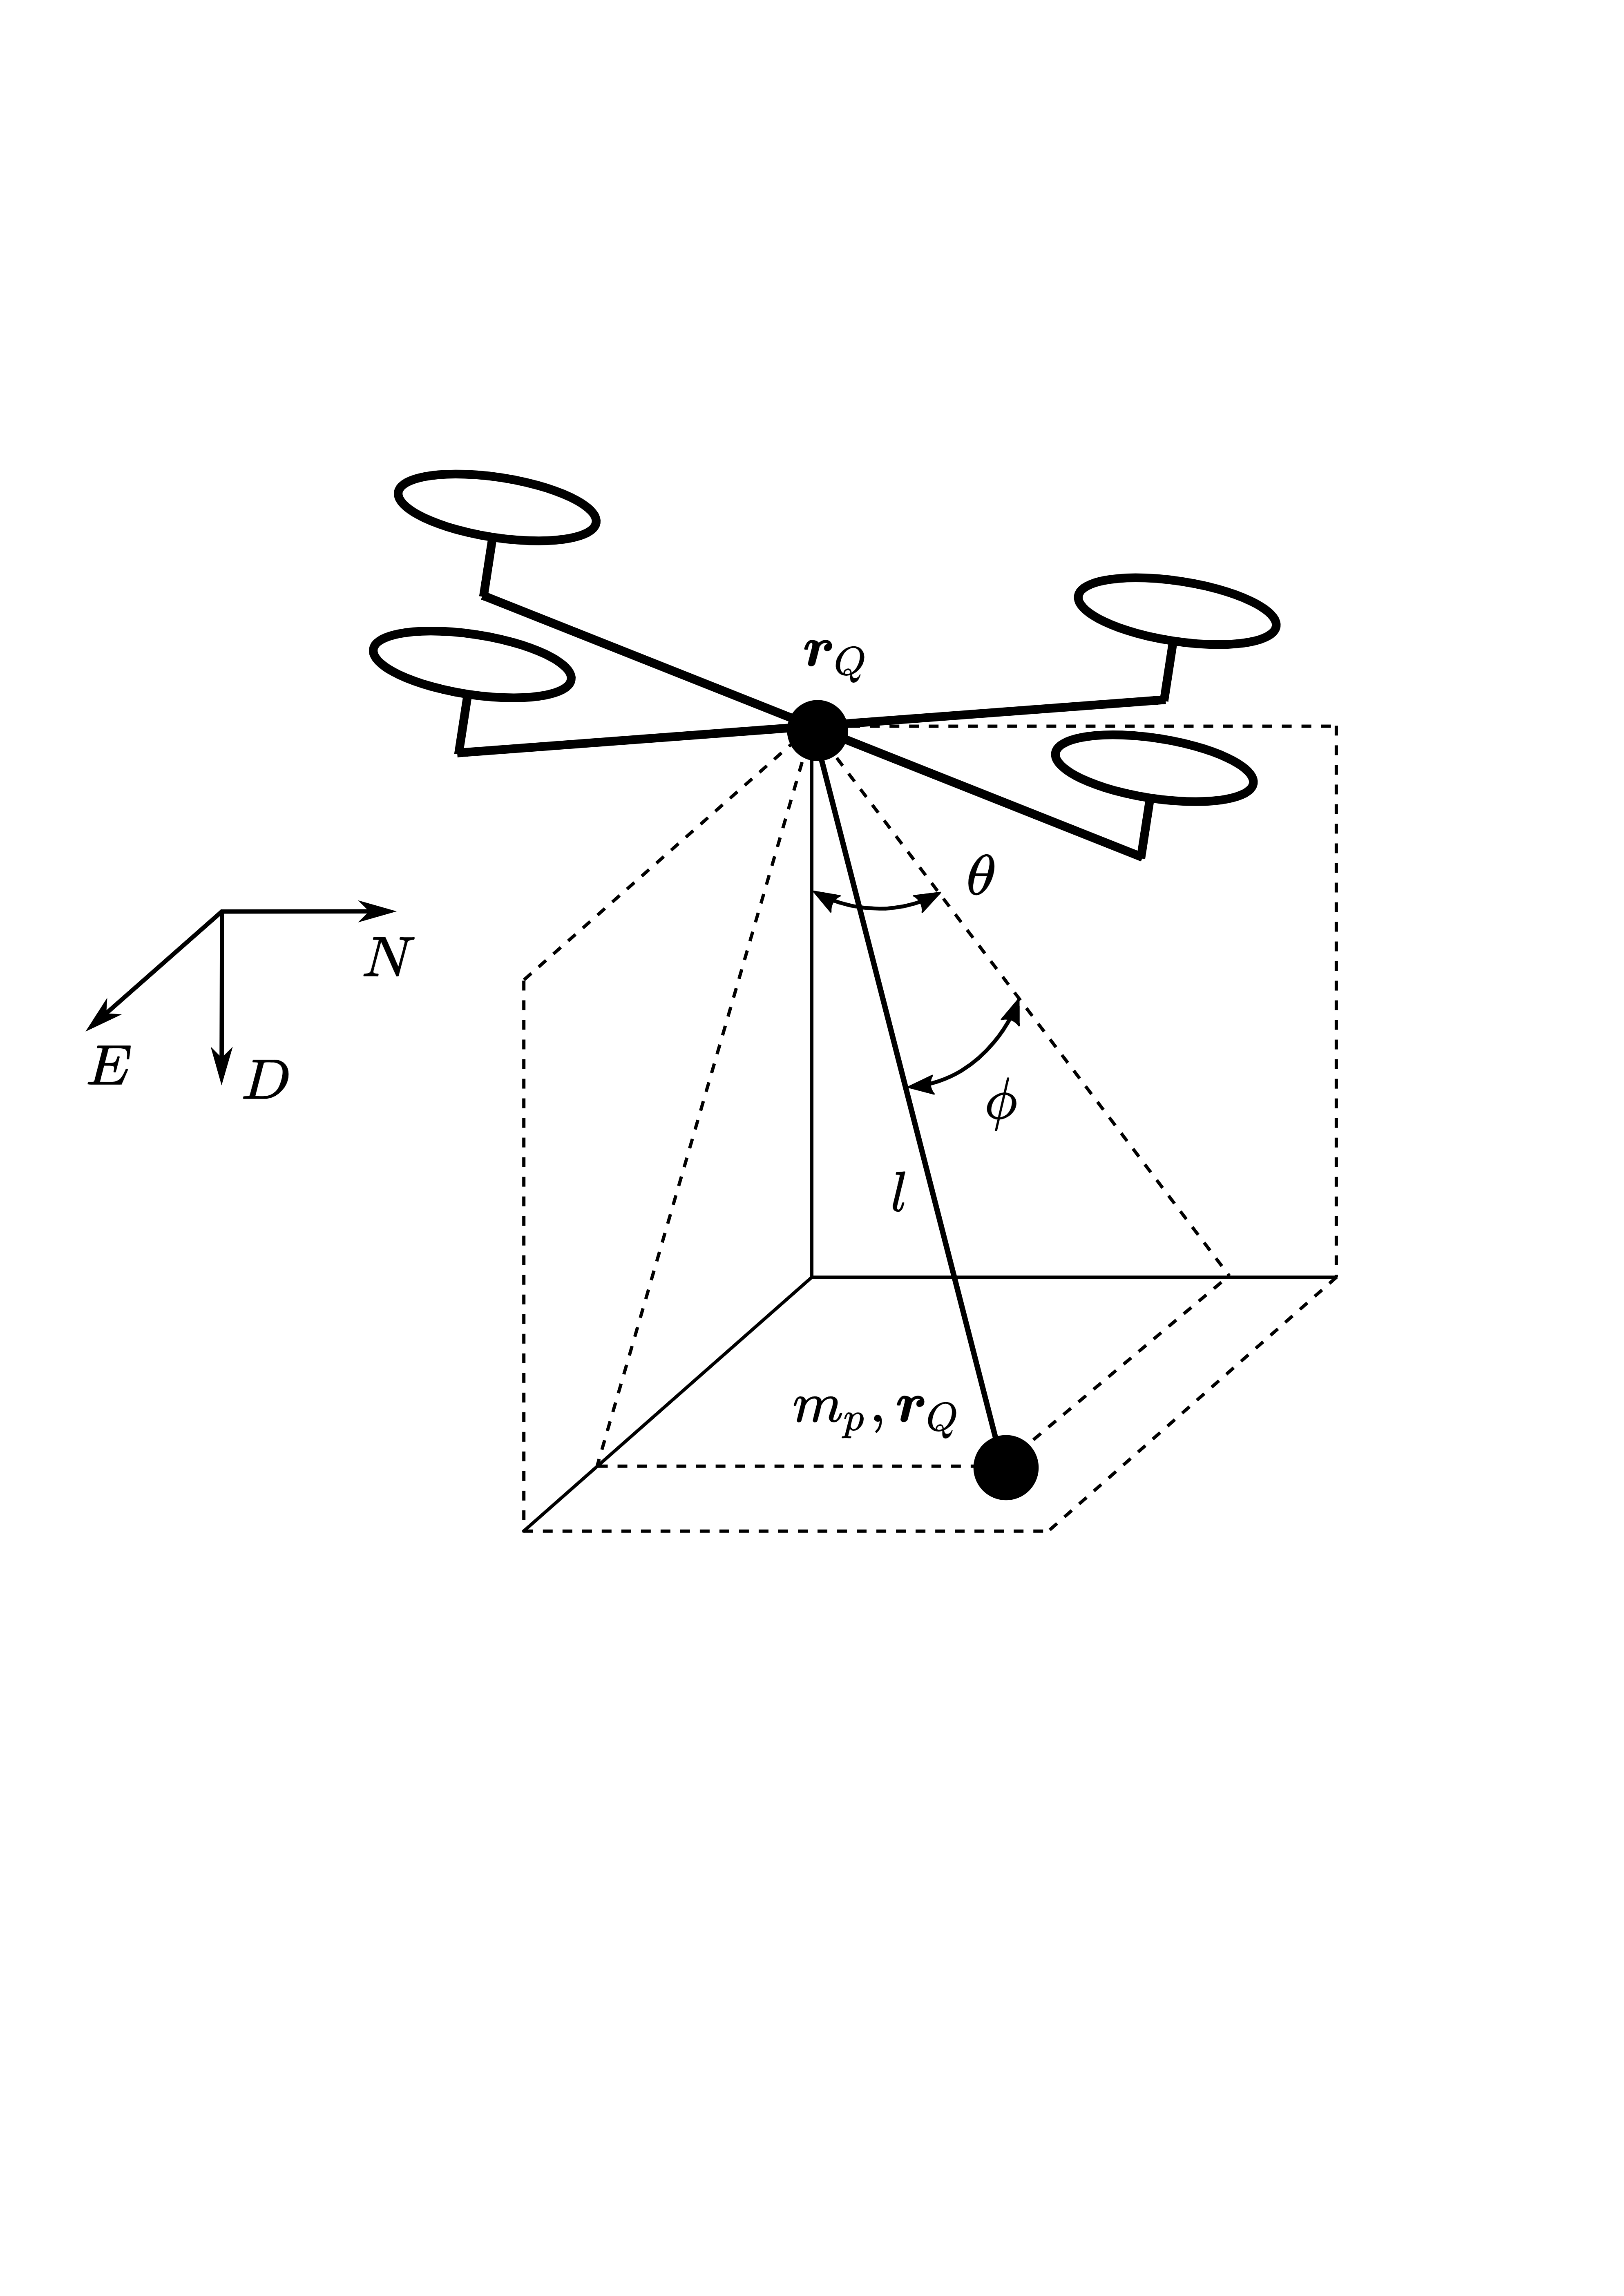
\includegraphics[width=0.6\linewidth]{modelling/fig/quad_with_payload.png}
        \caption{Schematic of a multirotor with suspended payload from \cite{Slabber2020}}
        \label{fig:quad_with_payload}
    \end{figure}

    \subsection{Payload assumptions} \label{sec:payload_assumptions}

        \paragraph
        The following major assumptions are made regarding the payload model:
        \begin{itemize}
            \item The payload is a point-mass.
            \item The link is massless.
            \item The link is rigid.
            \item The link is attached to the \gls{CoM} of the multirotor.
        \end{itemize}

        \paragraph
        The payloads used in the practical setup described in Chapter~\ref{chap:exp_design}, 
        are small relative to the multirotor and the attachment point is close to the payload \gls{CoM}.
        They are attached with a low-friction joint to the suspended cable, therefore the rotation of the payload around the cable axis has a negligible effect on the multirotor. 
        Therefore modelling the payload as a point-mass appears to be a reasonable approximation.

        \paragraph
        The cables used in Chapter~\ref{chap:exp_design} have a low mass in comparison to the payloads and have a negligible amount of stretch.
        The cable remains straight and rigid during flight due to the tension applied by the payload.
        Aggressive manoeuvres may cause periods of zero cable tension where the load is in free-fall and the cable is slack \cite{Tang2015}.
        However, such aggressive manoeuvres are not considered in this work and the assumption of a rigid, massless cable appears reasonable.

        \paragraph
        In the practical setup shown in Chapter~\ref{chap:exp_design}, the cable attachment appears to be near to the \gls{CoM} of the multirotor.
        It is assumed that even if the attachment point is slightly below the actual \gls{CoM}, this has a negligible effect on the dynamics and can still be approximated by a \gls{CoM} attachment.
        Due to this assumption, the payload cannot apply a moment to the multirotor, hence the multirotor attitude dynamics is decoupled from the payload dynamics.
        Therefore, the multirotor can be modelled as a point-mass when considering the payload equations of motion.

    \subsection{Lagrangian}

        \paragraph
        Lagrangian mechanics is an energy-based modelling approach that can be used to derive differential equations describing a system \cite{Erasmus2020}.
        The dynamical equations of the suspended payload system were derived by \cite{Slabber2020} and the derivation in this work follows a similar approach.
        It is important to note that the derivation in this section considers the payload dynamics as a function of the motion of the multirotor \gls{CoM}.
        The derivation starts by defining the payload position as a function of the multirotor position in the inertial frame as,
        \begin{equation}
            \bm{r}_p = 
            \begin{bmatrix}
                x_p \\
                y_p \\
                z_p
            \end{bmatrix} = 
            \begin{bmatrix}
                x_Q + l \cos \phi \sin \theta \\
                y_Q +   \sin \phi \\
                z_Q + l \cos \phi \cos \theta
            \end{bmatrix} ,
        \end{equation}
        where $g$ is the acceleration due to gravity.
        The vector of generalised coordinates, $\bm{p}$, of the system can now be defined as,
        \begin{equation} \label{eq:general_coords}
            \bm{p} = 
            \begin{bmatrix}
                x_p \\
                y_p \\
                z_p \\
                \phi \\
                \theta
            \end{bmatrix}.
        \end{equation}

        \paragraph
        The kinetic energy, $\mathcal{T}_p$, and potential energy, $\mathcal{V}_p$, of the payload can be determined as,
        \begin{align}
            \mathcal{T}_p &= \frac{1}{2} m_p | \bm{\dot{r}}_p | ^2, \mbox{~~and~~} \\
            \mathcal{V}_p &= - m_p g z_p .
        \end{align}
        Note that these energy equations describe the system modelled as two point-mass bodies and do not consider the attitude dynamics of the multirotor.
        The Lagrangian can now be determined as,
        \begin{equation}
            \mathcal{L} = \mathcal{T}_p - \mathcal{V}_p .
        \end{equation}

    \FloatBarrier\subsection{Non-conservative forces}

        \paragraph
        Non-conservative forces and moments refer to effects that add or remove energy from the system.
        The non-conservative forces and moments acting on the payload include the aerodynamic drag force acting on the payload and the moment caused by the friction of the cable attachment.
        It is assumed that the cable is thin and short enough that the aerodynamic drag force acting on the cable is negligible.
        
        \paragraph
        According to the aerodynamic model presented in Equation~\ref{eq:drag_quad}, 
        the aerodynamic drag forces acting on the payload in the inertial frame are defined as,
        \begin{equation}
            \bm{F}_p^A = 
            \begin{bmatrix}
                F_{p_x}^A \\
                F_{p_y}^A \\
                F_{p_z}^A
            \end{bmatrix} = 
            \begin{bmatrix}
                \frac{1}{2} \phantom{.} \rho \phantom{.} C_{p} \phantom{.} \dot{x_p}^2 \\
                \frac{1}{2} \phantom{.} \rho \phantom{.} C_{p} \phantom{.} \dot{y_p}^2 \\
                \frac{1}{2} \phantom{.} \rho \phantom{.} C_{p} \phantom{.} \dot{z_p}^2
            \end{bmatrix}  \mbox{,} \label{eq:payload_drag_inertial}
        \end{equation}
        where $C_p$ is the lumped aerodynamic drag coefficient and reference area of the payload.
        It is assumed that the lumped payload drag coefficients are equal in all three axes, hence it is described by a single coefficient.

        % \paragraph
        % The actuator thrust force was derived in Equation~\ref{eq:thurst_force_moment} for the body frame.
        % This is transformed in the inertial frame with the \gls{DCM} as,
        % \begin{equation}
        %     \bm{F}_\mathcal{I}^T = \bm{R}_V^{-1} \bm{F}_\mathcal{B}^T .
        % \end{equation}

        \paragraph
        Friction at the cable attachment is modelled as linear damping.
        It is assumed that the coefficient of friction is equal in each axis of rotation.
        Therefore, the friction moments opposing the $\theta$ and $\phi$ rotations are given by,
        \begin{align}
            M_{\theta}^F  &= - c \dot{\theta} \\
            M_{\phi}^F    &= - c \dot{\phi}
        \end{align}
        respectively, where $c$ is the rotational friction coefficient for $\theta$ and $\phi$ rotations.
        A vector, $\bm{Q}$, of non-conservative forces and moments corresponding to the system coordinates in $\bm{p}$ can now be defined as,
        \begin{equation}
            \bm{Q} = 
            \begin{bmatrix*}[c]
                - F_{p_x}^A \\
                - F_{p_y}^A \\
                - F_{p_z}^A \\
                M_{\theta}^F - F_{p_y}^A \cos{\phi} \\
                M_{\phi}^F - F_{p_x}^A \cos{\theta}
            \end{bmatrix*}.
        \end{equation}

        % ?? Check of dit reg is. Dalk nie conservative forces of multirotor nie

        % ?? Check element wise multiplication equations

    \FloatBarrier\subsection{Equations of motion}
    
        \paragraph
        The set of Euler-Lagrange equations for this system are described by,
        \begin{equation}
            \frac{d}{dt}\left(\frac{\partial\mathcal{L}}{\partial\dot{p_j}}\right) - \frac{\partial\mathcal{L} }{\partial p_j} = Q_j,
        \end{equation}
        where 
        $p_j$ is an element in $\bm{p}$,
        $Q_j$ is the corresponding element in $\bm{Q}$,  and
        $j = \{1,~2,~3,~4,~5\}$.
        This set of coupled equations was solved with the Symbolic Maths Toolbox\texttrademark~\cite{SymbolicToolbox2021} in MATLAB to determine the payload equations of motion. 
        This yields a set of \glspl{ODE} in the form,
        \begin{equation} \label{eq:payload_odes}
            \ddot{\bm{p}} = f( \dot{\bm{p}}, \bm{p}, \ddot{\bm{r}}_Q, \dot{\bm{r}}_Q) ,
        \end{equation}
        which describes the motion of the payload as a function of the motion of the multirotor \gls{CoM} in the inertial frame.

        % ?? Maybe add odes in appendix
        % ?? Check in MATLAb if dot{r_Q} really in dynamics
        % ?? Discuss weak link between altitude dynamics and swing angle

    \FloatBarrier\subsection{Payload forces acting on the multirotor}

        \paragraph
        % The set of \glspl{ODE} in Equation~\ref{eq:payload_odes} can be manipulated into the form,
        % \begin{equation}
        %     \ddot{\bm{r}}_Q,p = f( \dot{\bm{p}}, \bm{p}, \ddot{\bm{r}}_Q, \dot{\bm{r}}_Q) ,
        % \end{equation}
        % where 
        % where describes the component of the acceleration of the multirotor as a function of the motion
        The reaction force applied to the multirotor due to the payload can now be determined in the inertial frame as,
        \begin{equation}
            \bm{F}_{\mathcal{I}}^P = m_Q \ddot{\bm{r}}_Q ,
        \end{equation}
        from Newton's second law, where $\ddot{\bm{r}}_Q$ represents the component of the multirotor acceleration caused by the suspended payload.
        This force can be represented in the body frame as,
        \begin{equation}
            \bm{F}_{\mathcal{B}}^P = \bm{R}_V \bm{F}_{\mathcal{I}}^P .
        \end{equation}

        \paragraph
        The set of \glspl{ODE} represented by Equation~\ref{eq:payload_odes} provides a coupling between the multirotor and payload dynamics.
        The multirotor-payload system can now be simulated from a given initial condition with an \gls{ODE} solver in Simulink\texttrademark.
    
    % \FloatBarrier\section{Linearised model} \label{sec:linear_model}
        
    %     \paragraph
    %     The dynamical equations derived in previous sections present a non-linear model of the multirotor-payload system.
    %     However, a linearised state-space model of this system is required for \gls{LQR} control, which will be discussed in Section~\ref{sec:lqr}.
    %     The \gls{LQR} controller and linear model derived by \cite{Slabber2020} will be discussed in this section and used in this work.
    %     This controller is used for North velocity control of a multirotor with a suspended payload.

    %     \begin{figure}[htb]
    %         \centering
    %         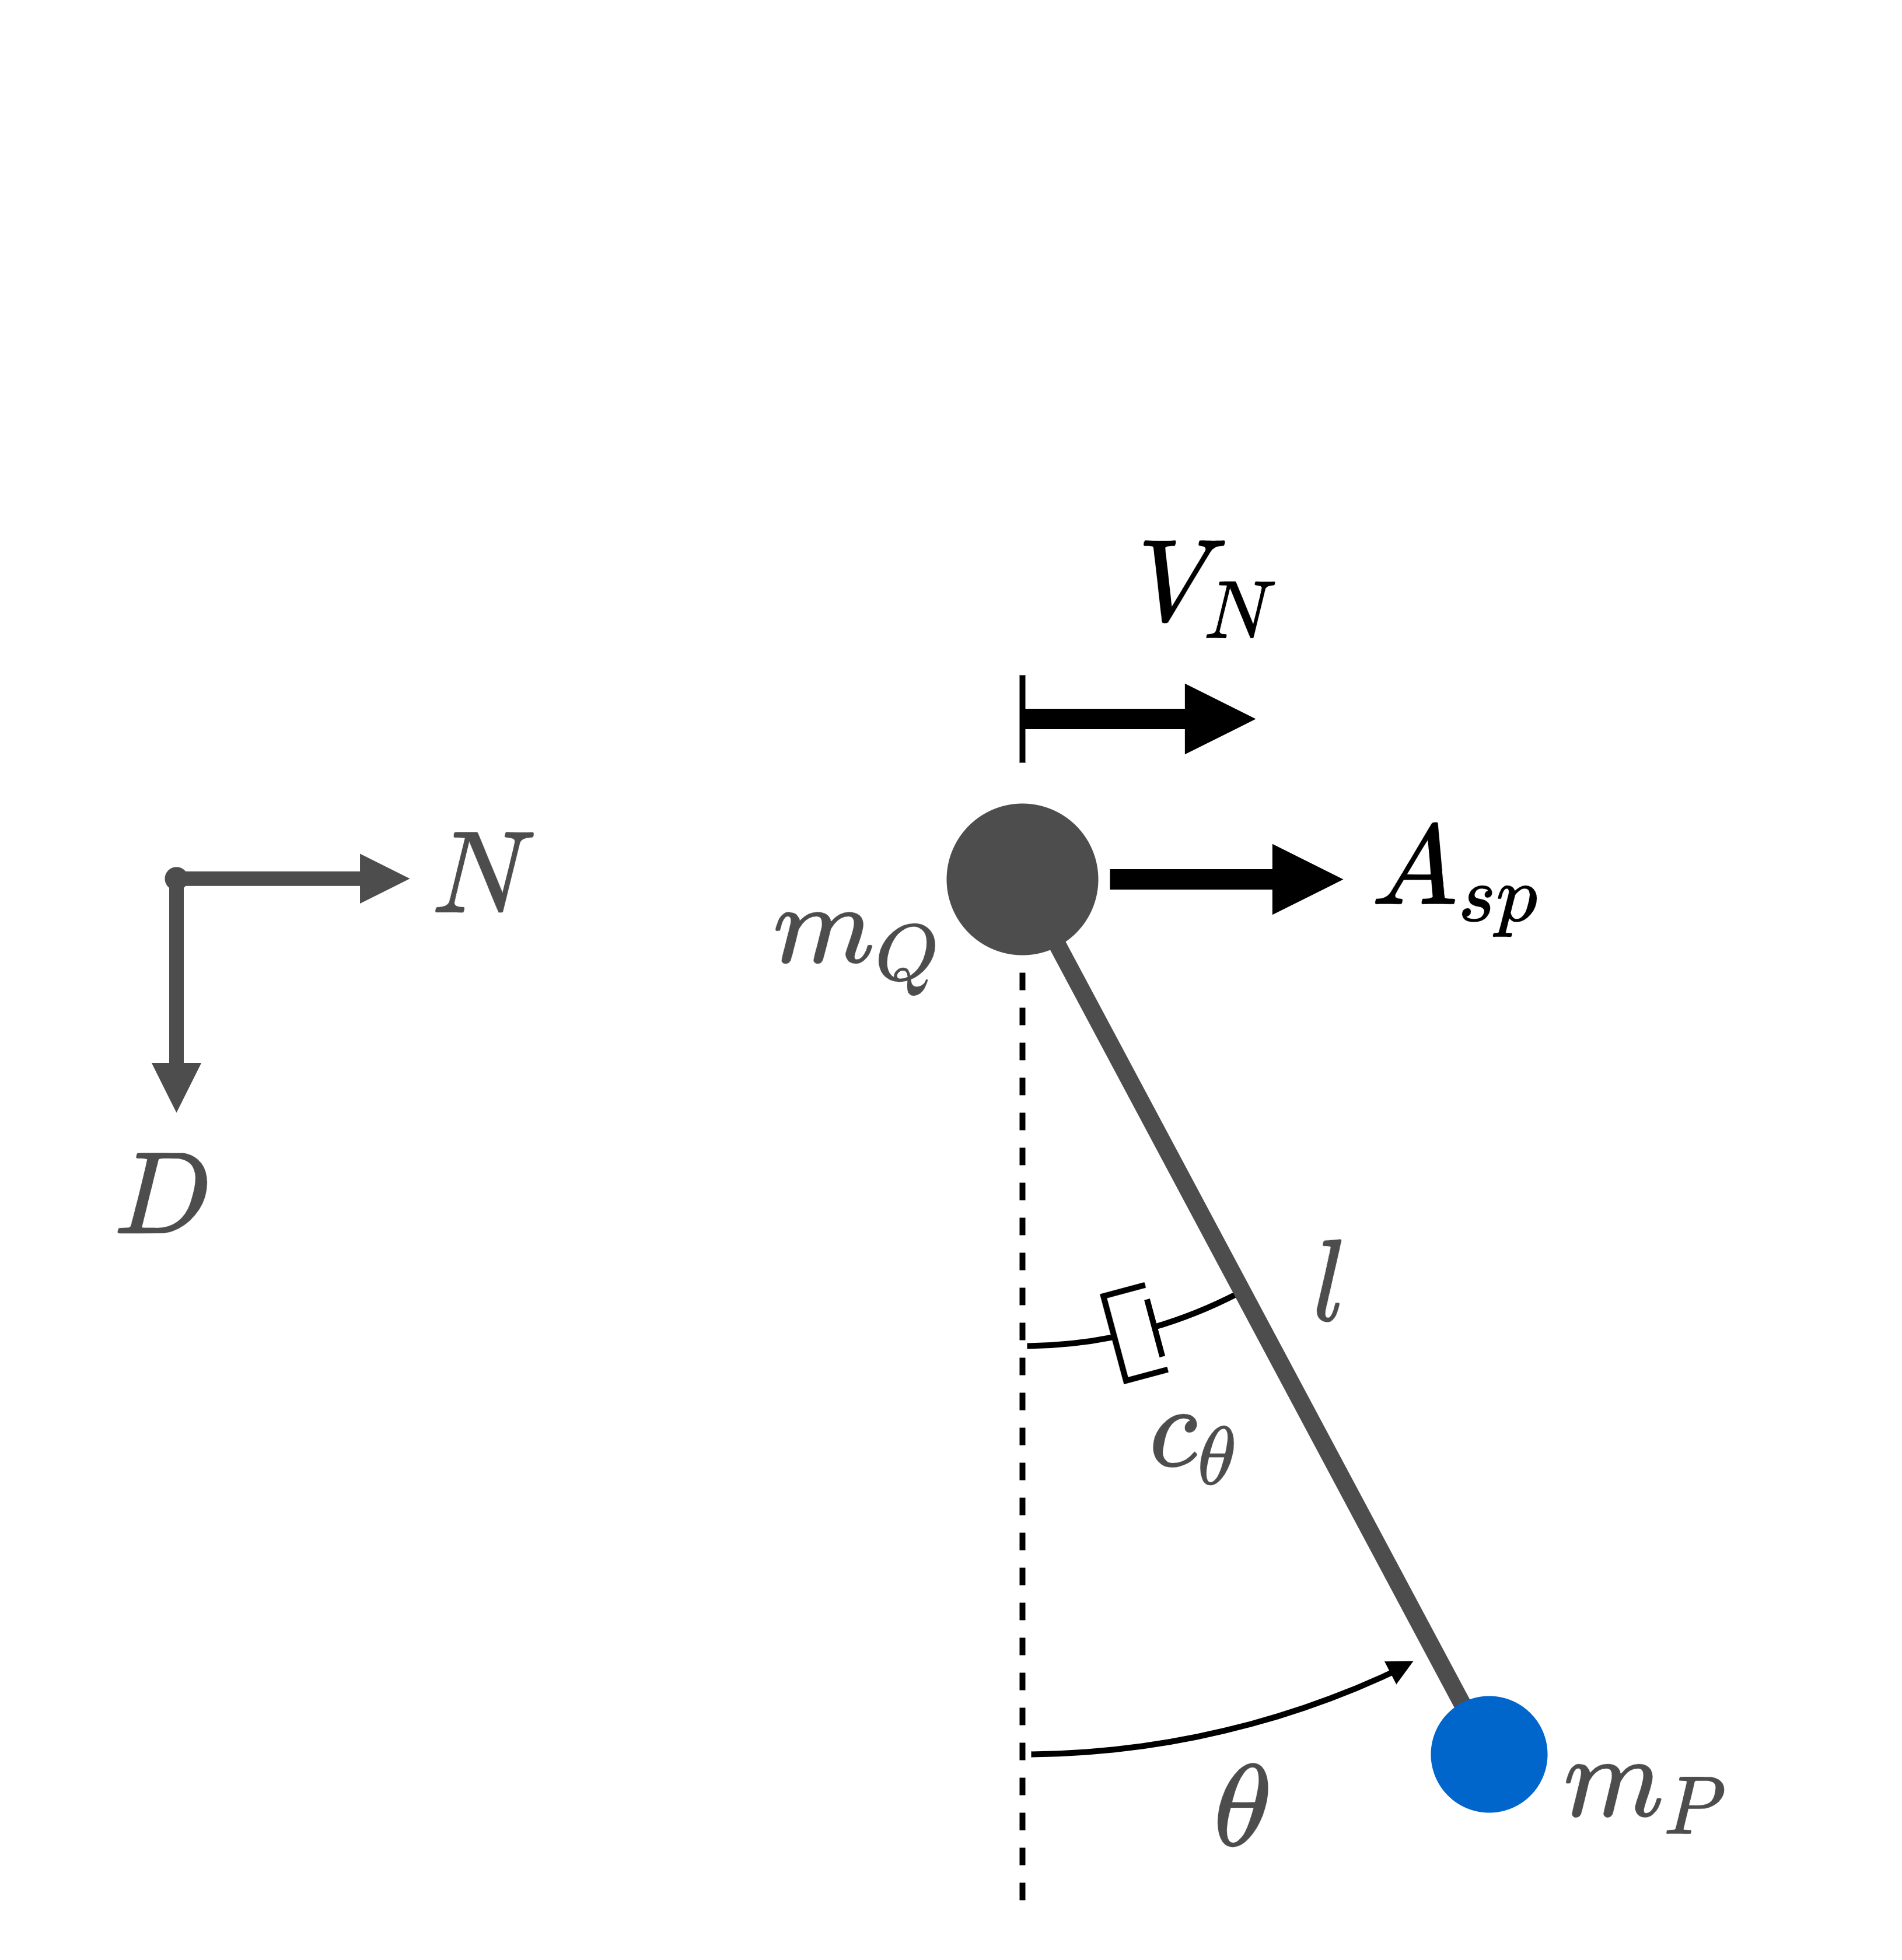
\includegraphics[width=0.45\linewidth]{modelling/fig/lqr_pend_diagram}            
    %         \caption{Schematic of a floating pendulum model considered for a North velocity controller}
    %         \label{fig:lqr_pend_diagram}
    %     \end{figure}

    %     \paragraph
    %     Figure~\ref{fig:lqr_pend_diagram} shows
    
    % \FloatBarrier\section{Dynamic payloads}
    
    %     In this work, a dynamic payload refers to a payload with dynamics that differ significantly from a rigid mass.
    %     When considering suspended payloads, a dynamic payload induces dynamics which differ from that of a simple pendulum.
    
    %     \begin{itemize}
    %         \item Most control in literature model payload as rigid Mass. Give references.
    %         \item Some add spring stiffness of cable (give references e.g. QuadLoad ElasticCable Prasanth Kotaru)
    %         \item but not practical because can design which cable you used. Cannot design which payload needs to be transported
    %         \item water looks like double payload
    %     \end{itemize}
    % % https://hybrid-robotics.berkeley.edu/publications/ACC2017_QuadLoad_ElasticCable.pdf), 
    % % https://www.researchgate.net/publication/352394086_A_Hybrid_Control_Approach_for_the_Sw[…]=publicationTitle&_iepl%5BtargetEntityId%5D=PB%3A352394086
    
    
\FloatBarrier\section{Model verification} \label{sec:model_verification}

    \paragraph
    To verify whether the non-linear simulation model derived in previous sections is an accurate representation of the real-world dynamics, the simulation data is verified against practical data.
    Firstly, a North velocity step response was performed in a practical flight with a multirotor to verify the multirotor model without a payload.
    The practical multirotor is described in Chapter~\ref{chap:exp_design}.
    % For simplicity in comparison, the body $\bar{\bm{x}}_{\mathcal{B}}$ axis was aligned with the inertial North axis for this flight.
    
    \paragraph
    This flight was performed on a day with almost no wind to minimise the effect of wind disturbances in the comparison.
    Starting from the same initial condition, a velocity step setpoint was commanded in a simulation and the resulting simulation data was compared to the practical flight data.
    This Simulink\texttrademark~simulation environment is discussed in Chapter~\ref{chap:control} and includes the dynamics of the default multirotor controllers.
    The results compare the combined multirotor and controller simulation model to the practical flight data.

    \begin{figure}[htb]
    \centering
    \begin{tikzpicture}
        \begin{axis}[            
            xlabel = Time,
            ylabel = North velocity,
            x unit = \si{\second},
            y unit = \si{\metre/\second},
            xmin = 0,   xmax = 16,
            ymin = -0.1,  ymax = 2.5,
            grid = major,
            legend cell align = left,
            legend pos = south east,
            grid style = dashed,
            legend style = {font = \scriptsize},
            label style = {font = \scriptsize},
            tick label style = {font = \scriptsize},
            width = 0.95\columnwidth,
            height = 0.5\columnwidth,
            % initialize Dark2
            cycle list/Dark2,
            % combine it with 'mark list*':
            cycle multiindex* list = {
                Dark2\nextlist
            }
        ]
                
        \addplot+[mark = none, style = solid, ultra thick] 
        table[x = time, y = vel_sp, col sep = comma] 
        {modelling/csv/prac_vs_sim_vel_step_Simulink_2021-08-20_04_no_load_velocity_steps_wind_0.5.csv.csv};
        \addlegendentry{$V_{N_{sp}}$}

        \addplot+[mark = none, style = solid, ultra thick] 
        table[x = time, y = vel.prac, col sep = comma] 
        {modelling/csv/prac_vs_sim_vel_step_Simulink_2021-08-20_04_no_load_velocity_steps_wind_0.5.csv.csv};
        \addlegendentry{$V_N$ (Practical)}

        \addplot+[mark = none, style = dashed, ultra thick] 
        table[x = time, y = vel.sim, col sep = comma] 
        {modelling/csv/prac_vs_sim_vel_step_Simulink_2021-08-20_04_no_load_velocity_steps_wind_0.5.csv.csv};
        \addlegendentry{$V_N$ (Simulated)}

        \end{axis}
    \end{tikzpicture} 
    \caption{Comparison of simulated and practical data from Honeybee.}
    \label{fig:prac_vs_sim_vel_step_no_payload}
\end{figure}


    \paragraph
    Figure~\ref{fig:prac_vs_sim_vel_step_no_payload} shows the velocity step responses of a practical and a simulated flight.
    From a visual inspection of the plots, it is clear that the velocity responses match well.
    Note that the practical velocity curve is slightly more irregular and not as smooth as the simulated curve.
    This may be due to slight wind disturbances or sensor noise, which are not considered in the simulation.

    \begin{figure}[htb]
    \centering
    \begin{tikzpicture}
        \begin{axis}[            
            xlabel = Time,
            ylabel = North velocity,
            x unit = \si{\second},
            y unit = \si{\metre/\second},
            xmin = 0,   xmax = 16,
            ymin = -0.1,  ymax = 2.8,
            grid = major,
            legend cell align = left,
            legend pos = south east,
            grid style = dashed,
            legend style = {font = \scriptsize},
            label style = {font = \scriptsize},
            tick label style = {font = \scriptsize},
            width = 0.95\columnwidth,
            height = 0.5\columnwidth,
            % initialize Dark2
            cycle list/Dark2,
            % combine it with 'mark list*':
            cycle multiindex* list = {
                Dark2\nextlist
            }
        ]
                
        \addplot+[mark = none, style = solid, ultra thick] 
        table[x = time, y = vel_sp, col sep = comma] 
        {modelling/csv/prac_vs_sim_vel_step_Simulink_2021-08-20_02_l-2_mp-0.3-wind-0.5.csv.csv};
        \addlegendentry{$V_{N_{sp}}$}

        \addplot+[mark = none, style = solid, ultra thick] 
        table[x = time, y = vel.prac, col sep = comma] 
        {modelling/csv/prac_vs_sim_vel_step_Simulink_2021-08-20_02_l-2_mp-0.3-wind-0.5.csv.csv};
        \addlegendentry{$V_N$ (Practical)}

        \addplot+[mark = none, style = dashed, ultra thick] 
        table[x = time, y = vel.sim, col sep = comma] 
        {modelling/csv/prac_vs_sim_vel_step_Simulink_2021-08-20_02_l-2_mp-0.3-wind-0.5.csv.csv};
        \addlegendentry{$V_N$ (Simulated)}

        \end{axis}
    \end{tikzpicture} 
    \caption{Velocity step comparison of simulated and practical data for Honeybee with a suspended payload.}
    \label{fig:prac_vs_sim_vel_step_with_payload}
\end{figure}


    \paragraph
    The same procedure was followed to verify the multirotor with a suspended payload model.
    Figure~\ref{fig:prac_vs_sim_vel_step_with_payload} compares the practical and simulated velocity step responses with a suspended payload attached to the vehicle.
    The shape of the velocity curves also match well in this comparison.
    However, they do not correlate as well as they do in the no-load experiment.
    This may be due to the added complexity of the model.
    The considered payload model adds modelling assumptions which add to the inaccuracy of the model.
    The system also considers many state variables that each need to be assigned an accurate initial condition value.
    Furthermore, the effect of wind disturbances is expected to be greater for the multirotor-payload system than for the multirotor without a load.

    \paragraph
    However, the shape of the practical and simulated velocity curves are still well matched.
    This seems to be an impressive result for such a complex system with numerous interlinking elements.
    Both systems provide an overshoot of a similar value.
    The amplitude and frequency of the velocity oscillations also appear to be very similar.

    \begin{figure}[htb]
    \centering
    \begin{tikzpicture}
        \begin{axis}[            
            xlabel = Time,
            ylabel = Payload angle,
            x unit = \si{\second},
            y unit = \si{\degree},
            xmin = 0,   xmax = 16,
            ymin = -20,  ymax = 20,
            grid = major,
            legend cell align = left,
            legend pos = south east,
            grid style = dashed,
            legend style = {font = \scriptsize},
            label style = {font = \scriptsize},
            tick label style = {font = \scriptsize},
            width = 0.95\columnwidth,
            height = 0.5\columnwidth,
            % initialize Dark2
            cycle list/Dark2,
            % combine it with 'mark list*':
            cycle multiindex* list = {
                Dark2\nextlist
            }
        ]
                
        \addplot+[mark = none, style = solid, ultra thick] 
        table[x = time, y = theta.prac, col sep = comma] 
        {modelling/csv/prac_vs_sim_vel_step_Simulink_2021-08-20_02_l-2_mp-0.3-wind-0.5.csv.csv};
        \addlegendentry{Practical}

        \addplot+[mark = none, style = dashed, ultra thick] 
        table[x = time, y = theta.sim, col sep = comma] 
        {modelling/csv/prac_vs_sim_vel_step_Simulink_2021-08-20_02_l-2_mp-0.3-wind-0.5.csv.csv};
        \addlegendentry{Simulated}

        \end{axis}
    \end{tikzpicture} 
    \caption{Payload angle comparison of simulated and practical data for Honeybee with a suspended payload}
    \label{fig:prac_vs_sim_theta_with_payload}
\end{figure}


    \paragraph
    Figure~\ref{fig:prac_vs_sim_theta_with_payload} shows the payload angle for the same flight as Figure~\ref{fig:prac_vs_sim_vel_step_with_payload}.
    It is clear that the payload angle response of the simulated system matches the practical data well. 
    
\section{Summary}

    \paragraph
    This chapter showed a detailed derivation of a mathematical model representing the Honeybee multirotor with a suspended payload.
    A comparison of the simulation model and practical flight data showed that the model provides a good representation of the of the actual multirotor-payload system.
    The mathematical model derived in this chapter can therefore be used for further simulations in subsequent chapters.

% ?? Add summary of each chapter

}